Die Erreichbarkeitskarte ist eine Erweiterung der Umgebungskarte und wird bei der Planung des eigenen Wegs erstellt. Sie gibt für jeden Zeitpunkt Auskunft, welche Zellen mit wie vielen Wegschritten von der aktuellen Position aus erreichbar sind. Da nicht davon auszugehen ist, dass ein Agent eine Zelle in einem Zeitschritt vollständig verlässt und die benachbarte Zelle vollständig betritt, muss der planende Agent seine Bewegungsschritte für \(t\) und \(t + 1\) reservieren. Das hat zur Folge, dass Agenten nicht direkt hintereinander fahren können und ist einer der beiden Mechanismen, wie Kollisionen zwischen den Agenten verhindert werden. \cite{book:regele}
\begin{figure}[H]
    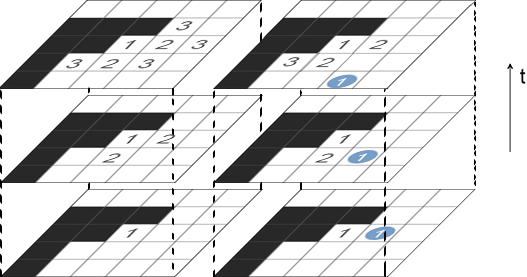
\includegraphics[width=9cm]{images/extended_occupancy.png}
    \centering
    \caption{Beispiele für eine Erreichbarkeitskarte}
    \label{fig:extended_occupancy}
\end{figure}
Abbildung \ref{fig:extended_occupancy} zeigt zwei Erreichbarkeitskarten. Für die linke Karte sind keine Agenten eingetragen. In der rechten Karte ist der geplante Weg für Agent "'1"' eingetragen (in der Abbildung blau). Im Vergleich zeigt sich, dass wegen des Sicherheitsabstand nach zwei Zeitschritten auf der rechten Karte weniger Zellen erreicht werden können.